
%\usepackage[subtle]{savetrees}
%\usepackage[margin=2cm]{geometry}
\usepackage{tikz,amsmath, amssymb,bm,color, amsthm,amsfonts}
\usetikzlibrary{positioning, calc,chains,fit,shapes}
%\usetikzlibrary{circuits.logic.US,circuits.logic.IEC,fit}
\usepackage{enumerate}
\usepackage{comment}
\usepackage{tikz}
\usepackage{graphics}
%\usepackage[cm]{fullpage}
\usepackage{longtable}
\usepackage{mdframed}
\usepackage{caption}
\usepackage{subcaption}
\usepackage{slashbox}
\usepackage{url}
\usepackage{framed}
\usepackage{array}
\usepackage{tabu}
\usepackage{lscape}
\usepackage{multirow}
\usepackage{ulem}
\usepackage{multicol}
\usepackage{placeins}
\usepackage{cite}
\usepackage{enumitem}
\usepackage{mathtools}
%\usepackage[numbers]{natbib}
%\usepackage{mathtools}
%\usepackage{authblk}

\mdfsetup{skipabove=2pt,skipbelow=2pt}
%\setlenght {\marginparwidth }{2cm}
%\usepackage{todonotes}

%\usepackage{floatrow}
%\usepackage{adjustbox}
%\setlength{\extrarowheight}{.05ex}
%\renewcommand\thesubfigure{\roman{subfigure}}


%\newtheorem{theorem}{Theorem}[section]
%\newtheorem{lemma}[theorem]{Lemma}
%\newtheorem{observation}[theorem]{Observation}
%\newtheorem{corollary}[theorem]{Corollary}
%\newtheorem{proposition}[theorem]{Proposition}
%\newtheorem{definition}[theorem]{Definition}
\newtheorem{construction}{Construction}
%\newtheorem{conjecture}{Conjecture}
%\newtheorem{remark}[theorem]{Remark}

\newcommand{\pname}[1]{\textnormal{\textsc{#1}}}
\newcommand{\cclass}[1]{\textnormal{\textsf{#1}}}
\newcommand{\nog}{nine} % no of members in the gang!
\newcommand{\nogd}{nineteen} % no of members in the gang - for deletion/completion
\newcommand{\nogl}{eighteen} % no of members in the larger gang - for editing
\newcommand{\nogld}{thirty eight} % no of members in the larger gang - for deletion/completion
\newcommand{\diffnog}{ten} %
%\newcommand{\dominatedby}{dominated by} %
%\newcommand{\dominatingset}{dominating set} %
%\newcommand{\dominates}{dominates} %
\newcommand{\simulates}{simulates} %
\newcommand{\baseset}{base} %
\newcommand{\issimulatedby}{is simulated by} %

\newcommand{\StarSAT}{\pname{8-SAT$_{\geq 6}$}}
\newcommand{\FSAT}{\pname{4-SAT$_{\geq 2}$}}
\newcommand{\FISAT}{\pname{5-SAT$_{\geq 3}$}}
\newcommand{\SIXSAT}{\pname{6-SAT$_{\geq 4}$}}
\newcommand{\ESAT}{\pname{8-SAT$_{\geq 6}$}}
\newcommand{\KSAT}{\pname{$k$-SAT$_{\geq {k-2}}$}}
\newcommand{\KSATO}{\pname{$k$-SAT}}
\newcommand{\ESATO}{\pname{8-SAT}}
\newcommand{\FSATO}{\pname{4-SAT}}
\newcommand{\FISATO}{\pname{5-SAT}}
\newcommand{\TSAT}{\pname{3-SAT}}
\newcommand{\HED}{\pname{${H}$-free Edge Deletion}}
\newcommand{\AEE}{\pname{${A}$-free Edge Editing}}
\newcommand{\AED}{\pname{${A}$-free Edge Deletion}}
\newcommand{\TSED}{\pname{$t$-star-free Edge Deletion}}
\newcommand{\ATSED}{\pname{Annotated $t$-star-free Edge Deletion}}
\newcommand{\AFSED}{\pname{Annotated $4$-star-free Edge Deletion}}
\newcommand{\FSED}{\pname{$4$-star-free Edge Deletion}}
\newcommand{\FVSED}{\pname{$5$-star-free Edge Deletion}}
\newcommand{\HEE}{\pname{${H}$-free Edge Editing}}
\newcommand{\HEC}{\pname{${H}$-free Edge Completion}}
\newcommand{\HDEE}{\pname{${H'}$-free Edge Editing}}
\newcommand{\HDDEE}{\pname{${H''}$-free Edge Editing}}
\newcommand{\HDED}{\pname{${H'}$-free Edge Deletion}}
\newcommand{\HDEC}{\pname{${H'}$-free Edge Completion}}
\newcommand{\HBEE}{\pname{${\overline{H}}$-free Edge Editing}}
\newcommand{\HBED}{\pname{${\overline{H}}$-free Edge Deletion}}
\newcommand{\HBEC}{\pname{${\overline{H}}$-free Edge Completion}}
\newcommand{\HOEDCE}{\pname{${H_1}$-free Edge Deletion(Completion/Editing)}}
\newcommand{\HEDCE}{\pname{${H}$-free Edge Deletion(Completion/Editing)}}
\newcommand{\HEEDC}{\pname{${H}$-free Edge Editing(Deletion/Completion)}}
\newcommand{\HDEEDC}{\pname{${H'}$-free Edge Editing(Deletion/Completion)}}
\newcommand{\BFED}{\pname{Bow-free Edge Deletion}}
\newcommand{\ABFED}{\pname{Annotated Bow-free Edge Deletion}}
\newcommand{\DTIS}{\pname{Distance-3 Independent Set}}
\newcommand{\SVC}{\pname{Strong Vertex Cover}}
\newcommand{\CLIQUE}{\pname{Clique}}
\newcommand{\IS}{\pname{Independent Set}}
\newcommand{\PFS}{\pname{Propagational-$f$ Satisfiability}}
\newcommand{\RHED}{\pname{Restricted ${H}$-free Edge Deletion}}
\newcommand{\RHEC}{\pname{Restricted ${H}$-free Edge Completion}}
\newcommand{\RHDED}{\pname{Restricted ${H'}$-free Edge Deletion}}
\newcommand{\RHDEC}{\pname{Restricted ${H'}$-free Edge Completion}}
\newcommand{\RHEE}{\pname{Restricted ${H}$-free Edge Editing}}
\newcommand{\PH}{$\cclass{NP} \subseteq \cclass{coNP/poly}$}
\newcommand{\NOPH}{$\cclass{NP} \not\subseteq \cclass{coNP/poly}$}
\newcommand{\LG}{\mathcal{W}}
\newcommand{\LGD}{\mathcal{W}'}
\newcommand{\LGDD}{\mathcal{W}''}


%\let\oldvee\vee
\renewcommand\vee{\boxtimes}

\newcommand\addvmargin[1]{
  \node[fit=(current bounding box),inner ysep=#1,inner xsep=0]{};
}
\setlength{\fboxrule}{0pt}

\newcommand{\defstage}[2]{% PGD Version
  \hfill\\\smallskip\noindent%
  \begin{tabularx}{\textwidth}{|l X|}%
    \hline%
    \multicolumn{2}{|l|}{\textbf{#1}}\\%
    &#2\\\hline%
  \end{tabularx}%
%  \smallskip%
}
\setlength\extrarowheight{15pt}

\newcounter{rowcntr}[table]
\renewcommand{\therowcntr}{\thetable.\arabic{rowcntr}}

% A new columntype to apply automatic stepping
\newcolumntype{N}{>{\refstepcounter{rowcntr}\therowcntr}c}

% Reset the rowcntr counter at each new tabular
\AtBeginEnvironment{longtabu}{\setcounter{rowcntr}{0}}

\newcounter{rowcntra}[table]
\renewcommand{\therowcntra}{\arabic{rowcntra}}

% A new columntype to apply automatic stepping
\newcolumntype{M}{>{\refstepcounter{rowcntra}\therowcntra}c}

% Reset the rowcntr counter at each new tabular
\AtBeginEnvironment{tabular}{\setcounter{rowcntra}{0}}

\newcommand{\NPC}{NP-Complete}


\newcommand{\highlight}[1]{\textcolor{blue}{#1}}
\newcommand{\dhanya}[1]{\textcolor{blue}{dhanya: #1}}


%\newcommand{\XCD1}[1]{\pname{$\chi_{cd}$\ensuremath{(#1)}}}
\newcommand{\XCD}{\pname{$\chi_{cd}$}}
\newcommand{\SC}{\pname{$\omega_{s}$}}

\newcommand{\CDC}{\textsc{CD-coloring}}
\newcommand{\SCP}{\textsc{Separated-Cluster}}
\newcommand{\TD}{\textsc{Total Domination}}
\newcommand{\ISP}{\textsc{Independent Set}}
\newcommand{\CC}{\textsc{Clique Cover}}
\newcommand{\TETHS}{Further, the problem cannot be solved in time \ensuremath{2^{o(|V(G)|)}}, unless the ETH fails}
%\usetikzlibrary{positioning,chains,shapes,calc}
\usetikzlibrary{fit}
\thispagestyle{empty}
\usetikzlibrary{
  graphs,
  graphs.standard
}
\setbeamertemplate{itemize item}{\textbullet}
% Define a boolean parameter
\newboolean{longtalk}
\setboolean{longtalk}{true} % Set to 'true' to show the slides, 'false' to hide them


\newcommand{\takeaways}{
\begin{itemize}
\item Decentralized exchanges are designed for \emph{passive} liquidity provision.
\item Fixed costs to participate in markets lead to different economies of scale for heterogeneous \textbf{LP}s.
\item If fragmented: high-fee pools tend to have lower execution, lower liquidity yields and higher adverse selection cost.
\item But, fragmentation can be efficient.
\end{itemize}

\begin{center}
\begin{tabular}{ll}
\toprule
Low-fee pools & High-fee pools \\
\cmidrule{1-2}
High trading volume & Low trading volume \\
Low aggregate liquidity & High aggregate liquidity \\
Few, large \textbf{LP}s & Many, small \textbf{LP}s \\
Short liquidity cycles & Large liquidity cycles \\
\bottomrule
\end{tabular}
\end{center}

}

\begin{document}



\title[Liquidity fragmentation on decentralized exchanges]{Fragmentation and optimal liquidity supply \\ on decentralized exchanges}
\author[Lehar, Parlour, Zoican]{Alfred Lehar, Christine A. Parlour, and Marius Zoican}

\date{May 2024}

\institute[U Toronto]{Haskayne School of Business, University of Calgary \and Haas School of Business, UC Berkeley \and Rotman School of Management,  University of Toronto}

\begin{frame}[noframenumbering]
\titlepage
\end{frame}

\begin{frame}{Decentralized exchanges (DEX) trade}
    \begin{center}
        % Figure removed
    \end{center}
\end{frame}

\begin{frame}{DEX can provide better liquidity than centralized exchanges}
    \begin{center}
        % Figure removed
    \end{center}
\end{frame}

\begin{frame}\frametitle{What do we do?}
\begin{itemize}
\item Use the design of  an automated market maker (AMM) as a laboratory: 
\medskip
\begin{itemize}
\item[\textbullet] Study the effect of fixed and variable costs on liquidity supply
\smallskip
\item[\textbullet] Argue fragmented liquidity can be beneficial to capture passive liquidity supply. 
\end{itemize}
\bigskip
\item Why study an AMM?
\smallskip
\begin{enumerate}
\item They process a large volume of transactions.
\smallskip
\item They seem to provide more liquidity than centralized limit order markets.
\smallskip
\item As real world assets (RWA) move to tokenization models, trading may migrate.
\smallskip
\item Costs/benefits to supplying liquidity is cleaner to observe than in centralized markets.
\end{enumerate}
\end{itemize}
\end{frame}

\begin{frame}\frametitle{Uniswap - Details}
\begin{itemize}
\item UniSwap is a decentralized protocol originally on the Ethereum Blockchain.
\begin{itemize}
\item[\textbullet] Each pool has two assets -- all trades are swaps
\end{itemize}
\bigskip
\item There are three versions of Uniswap (v1,v2,v3)
\medskip
\item Features common to all versions:
\begin{itemize}
\item[\textbullet] Agents choose to supply or demand liquidity
\item[\textbullet] Trade prices automatically calculated as a function of liquidity demand and supply.
\item[\textbullet] Only payoff for liquidity supplier is a \% fee paid by the liquidity demander.
\end{itemize}
\medskip
\item Unique to v3
\begin{itemize}
\item[\textbullet] Variable fees:  Each asset pair can trade in 1, 5, 30 or 100bps pools.
\item[\textbullet] Concentrated liquidity:  Liquidity suppliers can choose the price range over which they supply liquidity 
\end{itemize}
\end{itemize}
\end{frame}


% \begin{frame}\frametitle{Uniswap -- Liquidity Provision v2 \\ A Pool with Ethereum ``E'' and a token ``T''}

% \begin{minipage}{0.35\textwidth}%
% \begin{tikzpicture}
% \draw(0,1) circle(0.5in);
% \draw[thick,dashed](-1.15,0.45)--(1.15,0.45);
% \draw(0,1) node[above]{E};
% \draw(0,0.35) node[below]{T};
% \end{tikzpicture}
% \end{minipage} %
% \begin{minipage}{0.55\textwidth}%
% \begin{itemize}
% \item Liquidity suppliers deposit Eth and T

% \medskip
% \item Liquidity demander who buys the token, removes it from the pool and deposits Eth.
% \item Liquidity demander who sells the token, adds it to the pool and withdraws Eth.

% \bigskip
% \item Liquidity demanders pay a fixed, proportional fee which is passed through to the liquidity suppliers.

% \end{itemize}
% \end{minipage}

% \end{frame}


\begin{frame}{Unique to v3:  Concentrated Liquidity}
\begin{itemize}
    \item On Uniswap v3, liquidity providers can specify price limits on their positions.
    \item If the current pool price (e.g., ``midpoint'') is outside the range, the position does not earn fees.
    \item $\rightarrow$ incentive to re-price the position to capture fees.
\end{itemize}
    \begin{center}
        % Figure removed
    \end{center}
\end{frame}

\begin{frame}{Fixed cost of adjusting liquidity (gas fee) on Uniswap v3}
    \begin{center}
        % Figure removed
    \end{center}
\end{frame}


\begin{frame}\frametitle{Price impact to purchase $\tau$ tokens}

\begin{minipage}{0.25 \textwidth}
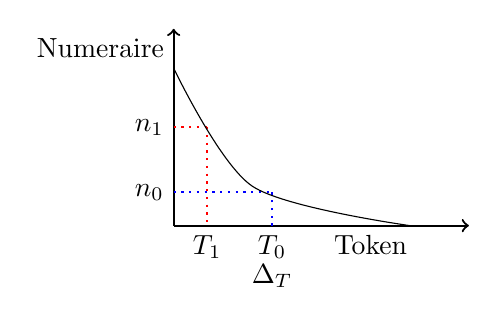
\begin{tikzpicture}[scale=0.25]
\draw[thick,->] (0,0)-- (15,0);
\draw[thick,->] (0,0) -- (0,10);
\draw (0,9) node[left]{Numeraire};
\draw(10,0) node[below]{Token};
\draw[dotted,red, thick](0,5)--(1.7,5);
\draw[dotted,red,thick](1.7,5)--(1.7,0);
\draw (0,1.7) node[left]{$n_0$};
\draw (1.7,0) node[below]{$T_1$};
\draw(5,0) node[below]{$ T_0$};
\draw(5,-1.5) node[below] {$\Delta_T$}; 
\draw[dotted,blue,thick](5,0)--(5,1.7);
\draw[dotted,blue,thick](0,1.7)--(5,1.7);
\draw(0,5) node[left]{$n_1$};
\draw plot[smooth] coordinates {(12,0)  (4,2) (0,8)};
\end{tikzpicture}
\end{minipage}
\begin{minipage}{0.15\textwidth}
\hspace{1in}
\end{minipage}
\begin{minipage}{0.5 \textwidth}
\begin{itemize}
\item For $ \tau\rightarrow 0$ the exchange between Eth and the Token is $\frac{N}{T}=v$.
\item For larger trades, the exchange rate is determined by a ``bonding curve.''
\end{itemize}
\end{minipage}

\begin{itemize}
\item For given $N$ and $T$, if liquidity is provided across prices $\left[\frac{v}{(1+r)^2},v(1+r)^2\right]$, you need to deposit $n\left(\tau\right)$ in the pool to remove $\tau$ tokens: \end{itemize}
\begin{eqnarray*}
    \underbrace{\left(T_k-\tau+\frac{L_k}{\sqrt{v}\left(1+r\right)}\right)}_\text{virtual token reserves}\underbrace{\left(T_k v + n\left(\tau\right) +  L_k\frac{\sqrt{v}}{1+r}\right)}_\text{virtual numeraire reserves}=L_k^2.
\end{eqnarray*}
\begin{itemize}
\item As more liquidity is supplied ($L_k \nearrow$), bonding curve shifts out.
\end{itemize}
\end{frame}

% \begin{frame}
% \frametitle{Managing liquidity on DEX is costly}
% \begin{center}
%    % Figure removed
% \end{center}
% \end{frame}


\begin{frame}{Liquidity Provision on a DEX}

\bigskip

    \begin{enumerate}
    \item Unique laboratory to study how transaction costs affect the market for liquidity. \vspace{0.05in}
        \item DEX  designed for \textbf{passive} liquidity provision. \vspace{0.05in}
        \item ``\emph{Set-it-and-forget-it}'' liquidity: i.e., what ETFs did for portfolio management. \vspace{0.05in}
        \item On v3 actively managing liquidity is costly:
            \begin{enumerate}
                \item \emph{gas price} from interacting with Ethereum blockchain. \vspace{0.05in}
                \item \emph{time/effort} to monitoring the position.
            \end{enumerate}
        \vspace{0.05in}
        \item How do passive liquidity suppliers manage adverse selection? \vspace{0.05in}
        %\item Economies of scale: small liquidity providers face higher relative costs.\vspace{0.05in}
         
    \end{enumerate}
    \medskip

\citet{demsetz1968}: ``the question that is relevant for efficiency is whether or not the cost is appropriately economized.''  

    
    \end{frame}

\begin{frame}{Related literature}
We contribute to: \vspace{0.1in}
    \begin{itemize}
       \item  a growing literature on decentralized exchanges \citep{LeharParlour2021, caparros2023blockchain, augustin2022reaching, kp2023dex, capponi2023price, CapponiJia2021, BarbonRanaldo2021, HasbrouckRiveraSaleh2022}. \vspace{0.1in}
       \item the literature on optimal routing for retail orders \citep{Battalio2016,Cimon2021, FoucaultMenkveld2008}. \vspace{0.1in}
       \item the literature on make/take fees on  liquidity provision \citep{foucault2013liquidity, YaoYe2018,LiWangYe2021}
       
    \end{itemize}
\end{frame}


\begin{frame}\frametitle{Results}

\vspace{0.1in}

\begin{alertblock}{Theory and  evidence of LP ``clienteles'' based on their scale:}
\bigskip

\begin{enumerate}
    \item Small LPs are more passive: fill rates $\downarrow$, but adverse selection \& rebalancing cost $\downarrow$. 
    \item Large LPs are more active: fill rates $\uparrow$, but adverse selection \& rebalancing cost $\uparrow$. 
    \item This segmentation can be efficient
\end{enumerate}


\end{alertblock}

\end{frame}

% \begin{frame}{Related literature}
% We contribute to: \vspace{0.1in}
%     \begin{itemize}
%        \item  a growing literature on decentralized exchanges \citep{LeharParlour2021, caparros2023blockchain, augustin2022reaching, kp2023dex, capponi2023price, CapponiJia2021, BarbonRanaldo2021, HasbrouckRiveraSaleh2022}. \vspace{0.1in}
%        \item the literature on optimal routing for retail orders \citep{Battalio2016,Cimon2021, FoucaultMenkveld2008}. \vspace{0.1in}
%        \item the literature on make/take fees on  liquidity provision \citep{foucault2013liquidity, YaoYe2018,LiWangYe2021}
       
%     \end{itemize}
% \end{frame}

\begin{frame}{Model}
\begin{block}{Asset and markets.} \begin{itemize}
    \item Token with expected value $v_t$ trades on two liquidity pools with fees $h>\ell>0$.
    \item Fixed cost $\Gamma>0$ of interacting with the pool (e.g., gas fee).
\end{itemize}
\end{block}

\begin{block}{Liquidity providers (\textbf{LP})}
\begin{itemize}
\item Risk-neutral
\item Post liquidity on at most one pool between prices $\frac{v_t}{\left(1+r\right)^2}$ and $v_t\left(1+r\right)^2$.
\item Token endowments $q_i$; $q_i$ follows an exponential distribution with scale $\lambda$.
\end{itemize}
\end{block}

\begin{block}{Liquidity takers}
\begin{itemize}
    \item Value shock $v\left(1+\tilde{\delta}\right)$, where $\tilde{\delta}$ has density $\phi\left(\delta\right)=\frac{1}{2\Delta \sqrt{1+\delta}} \; \; \text{ for } \delta\in\left[0,\Delta^2-1\right]$.
    \item With rate $\eta$, shock is {\color{red} common value} (news). Aggressive orders are arbitrageurs \textbf{A}. 
    \item Otherwise, shock is {\color{blue} private value}. Aggressive orders are liquidity traders \textbf{LT}.
\end{itemize}
\end{block}

\end{frame}

\begin{frame}{Optimal trade size: minimize price impact and fees}

\begin{equation*}\label{eq:optimal_trade_size}
    \tau^\star\left(\delta\right)=T_k\min\left\{1,\frac{1+r}{r}\max\left\{0,1-\sqrt{\frac{1+f_k}{1+\delta}}\right\}\right\}.
\end{equation*}


    \small
    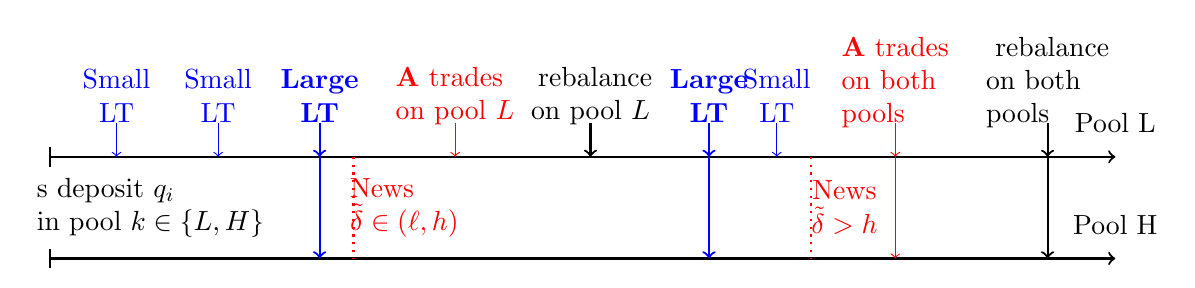
\begin{tikzpicture}[scale=0.86]
    % Draw the vertical lines
    \draw[|->, thick] (0,0) -- (15.75,0);
    \draw[|->, thick] (0,1.5) -- (15.75,1.5);

    \node at (15.75,0.5) {Pool H};
    \node at (15.75, 2) {Pool L};

    \node[align=left] at (1.5, 0.75) {$\LP$s deposit $q_i$ \\ in pool $k\in\left\{L,H\right\}$};

    \draw[->,blue] (1,2)--(1,1.5);
    \node[blue, align=center] at (1,2.4) {Small \\ LT};

    \draw[->,blue] (2.5,2)--(2.5,1.5);
    \node[blue, align=center] at (2.5,2.4) {Small \\ LT};

    \draw[->,blue,thick] (4,2)--(4,1.5);
    \draw[->,blue,thick] (4,1.5)--(4,0);
    \node[blue, align=center] at (4,2.4) {\bfseries Large \\ \bfseries LT};

    \draw[dotted,thick,red] (4.5,1.5) -- (4.5, 0);
    \node[red, align=left] at (5.25,0.75) {News \\ $\tilde{\delta}\in\left(\ell,h\right)$}; 

    \draw[->,red] (6,2)--(6,1.5);
    \node[red, align=left] at (6,2.4) {\textbf{A} trades \\ on pool $L$};

    \draw[->,thick](8,2)--(8,1.5);
    \node[align=center] at (8,2.4) {$\LP$ rebalance \\ on pool $L$};

    \draw[->,blue,thick] (9.75,2)--(9.75,1.5);
    \draw[->,blue,thick] (9.75,1.5)--(9.75,0);
    \node[blue, align=center] at (9.75,2.4) {\bfseries Large \\ \bfseries LT};


    \draw[->,blue] (10.75,2)--(10.75,1.5);
    \node[blue, align=center] at (10.75,2.4) {Small \\ LT};

    \draw[dotted,thick,red] (11.25,1.5) -- (11.25, 0);
    \node[red, align=center] at (11.75,0.75) {News \\ $\tilde{\delta}>h$}; 

    \draw[->,red] (12.5,2)--(12.5,1.5);
    \draw[->,red] (12.5,1.5)--(12.5,0);
    \node[red, align=left] at (12.5,2.6) {\textbf{A} trades \\ on both \\ pools};

    \draw[->,thick](14.75,2)--(14.75,1.5);
    \draw[->,thick](14.75,1.5)--(14.75,0);
    \node[align=left] at (14.75,2.6) {$\LP$ rebalance \\ on both \\ pools};

    
\end{tikzpicture}

\begin{itemize}
    \item Liquidity trades are immediately reversed by arbitrageurs \citep{LeharParlour2021}; \vspace{0.1in}
    \item News trades have permanent price impact. \vspace{0.1in}
    \item Large news trades ($\delta>(1+f_k)(1+r)^2-1$) exhaust available liquidity supply \\ $\Rightarrow$ costly re-balancing by \textbf{LP}s. \vspace{0.1in}
\end{itemize}

\end{frame}

\begin{frame}{Optimal order routing in practice}
    \begin{center}
        % Figure removed
    \end{center}
\end{frame}



\begin{frame}{Liquidity provider' choice}
Choose pool to maximize expected profit:
\begin{equation*}
    \max_{f\in\left\{\ell,h,\emptyset\right\}} q_i \left[\left(1-\eta\right) \mathcal{L}\left(f\right)-\eta \mathcal{A}\left(f\right)\right]-\eta \Gamma\left(1-\frac{\sqrt{1+f}\left(1+r\right)}{\Delta}\right),
\end{equation*}
where
\begin{itemize}
    \item $\mathcal{L}\left(f\right)$: liquidity yield on pool with fee $f$;
    \item $\mathcal{A}\left(f\right)$: adverse selection on pool with fee $f$;\vspace{0.1in}
\end{itemize}

    \begin{centering}
    % Figure removed
    \par\end{centering}
\end{frame}

\begin{frame}{Equilibrium regions}
    \begin{centering}
    % Figure removed
    \par\end{centering}
\end{frame}

\begin{frame}{Fragmented equilibrium}
\begin{itemize}
\item $\LP$s with endowment $\underline{q}_h$ do not supply liquidity.
\item There is a threshold endowment $\qmg$ such that all $\LP$s with $q_i>\qmg$ post liquidity on the low-fee pool and all $\LP$s with $q_i\leq \qmg$ choose the high-fee pool. Market share:
\begin{equation*}
w_\ell=\frac{\exp\left(-\frac{\qmg-\underline{q}_h}{\lambda}\right)\left(\qmg+\lambda\right)}{\underline{q}_h+\lambda} \leq 1,
\end{equation*}
\end{itemize}
\bigskip
% \begin{center}
% \begin{tikzpicture}[scale= 0.5]
%     \draw[thick] (0,0)--(15,0);
%     \draw[thick] (10,0)--(10,1);
%     \draw[thick] (15,0)--(15,1);
%     \draw[thick] (0,0)--(0,1);
%     \draw[thick] (5,0)--(5,1);
%     \draw[thick] node[below]{$1$};
%     \draw[thick] (5,0) node[below]{$\underline q$};
%     \draw[thick] (10,0) node[below]{$q_t$};
%     \draw[thick] (15,0) node[below]{Q};
%     \draw[thick] (2.5,0) node[above]{out};
%     \draw[thick] (7.5,0) node[above]{high};
%     \draw[thick] (12.5,0) node[above]{low};
% \end{tikzpicture}
% \end{center}
    \begin{centering}
    % Figure removed
    \par\end{centering}
\end{frame}


\begin{frame}{Gas cost and liquidity supply}
    \begin{centering}
    % Figure removed
    \par\end{centering}
\end{frame}

\begin{frame}\frametitle{Evaluating the fragmented liquidity}
\begin{block}{Proposition}
From any single fee pool, you can find a fragmented pool that increases the expected gains from trade, $\mathbb{E}\sum_k \delta T_k \tau^\star_k$.
\end{block}

\begin{enumerate}
    \medskip
\item Set the high fee equal to the single-pool fee: $h=f$ (same {\bfseries LP} participation).
\item Introduce a lower fee pool $\ell<h$ such that large {\bfseries LP} migrate there.
\bigskip
\end{enumerate}
    \begin{centering}
    % Figure removed
    \par\end{centering}
\end{frame}


\begin{frame}{Data}
\begin{itemize}
    \item Data from Uniswap v3 Subgraph on all trades, liquidity deposits and withdrawals from May 4, 2021 until July 15, 2023, including traders' wallet addresses. \vspace{0.1in}
    \item Gas cost is the average of the lowest daily 1000 gas prices for mint events. \vspace{0.1in}
    \item Focus on economically sizeable pools:
    \begin{enumerate}
        \item active in more than 100 days within the sample;
        \item 500+ liquidity events throughout the sample;
        \item average daily liquidity balance $>$US\$100,000;
        \item $>$1\% of volume for a traded pair.
    \end{enumerate} \vspace{0.1in}
    \item We obtain 274 pools in 242 asset pairs:
    \begin{enumerate}
        \item aggregate daily volume of US\$~1.12bn;
        \item end-of-sample aggregate liquidity US\$~2.53bn.
        \item account for 86.04\% of all Uniswap v3 interactions.
    \end{enumerate}
\end{itemize}
\end{frame}

\begin{frame}{Uniswap v3 pairs can be traded in 1, 5, 30, or 100 bps fee pools}
\begin{itemize}
    \item 32 fragmented pools collectively account for 95\% of committed liquidity and 93\% of traded volume
    \item Trading concentrates on adjacent fee levels e.g.:  \\ USDC/USDT 1-5bps, ETH/USDC 5-30bps, USDC-CRV 30-100bps
\end{itemize}
\bigskip
\begin{enumerate}
    \item Significant fragmentation across different-fee pools for the same pair.
    \item Low-fee pools are more actively traded, but high-fee pools are deeper.
    \begin{center}
        % Figure removed
    \end{center}
%\item We show that fixed transaction costs partly drive this effect.
\end{enumerate}
\end{frame}

\begin{frame}{Liquidity clienteles: high fee pools feature many small \textbf{LP}s.}
    \begin{center}
        % Figure removed
        % Figure removed
    \end{center}
\end{frame}

\begin{frame}{Low-fee pools: Larger mints, fewer LP wallets, many small trades.\\ (Mints and Trades in log USD)}
\begin{center}


\scalebox{0.73}{
\begin{tabular}{lccccccc}
\toprule
 & \multicolumn{1}{c}{Mint size} &  \multicolumn{1}{c}{Trade size} & \multicolumn{1}{c}{Volume} & \multicolumn{1}{c}{\# Trades}  & \multicolumn{1}{c}{\# Wallets} & \multicolumn{1}{c}{Liquidity yield} & \multicolumn{1}{c}{Price range} \\
 & (1) & (2) & (3) & (4) & (5) & (6) & (7) \\
\rowcolor{red!20} 
$ d_\text{low-fee}$ & 0.73*** & -0.30*** & 0.89*** & 1.02*** & -3.40*** & 2.03*** & -0.18*** \\
\rowcolor{red!20}
 & (12.27) & (-10.05) & (14.23) & (32.95) & (-5.00) & (3.60) & (-41.84) \\
Gas price $\times$ $ d_\text{low-fee}$ & 0.37*** & 0.08*** & -0.03 & -0.22*** & -3.00*** & 3.57** & -0.00 \\
 & (4.96) & (3.75) & (-0.95) & (-7.29) & (-3.43) & (2.30) & (-0.47) \\
Gas price $\times$ $ d_\text{high-fee}$ & 0.58*** & 0.17*** & 0.24*** & 0.07** & -2.89*** & 5.57*** & -0.03*** \\
 & (7.52) & (8.81) & (5.95) & (2.46) & (-3.15) & (2.83) & (-4.65) \\
Volume & 0.37*** & 0.16*** & 0.43*** & 0.20*** & 1.22*** & 1.01 & -0.01** \\
 & (8.68) & (21.38) & (15.27) & (13.85) & (6.56) & (0.81) & (-2.56) \\
Total value locked & -0.16 & 0.11*** & 0.23** & -0.01 & -1.86 & -13.42 & -0.02 \\
 & (-1.30) & (3.54) & (1.99) & (-0.18) & (-0.99) & (-1.09) & (-0.99) \\
Volatility & -0.04 & -0.01 & -0.07 & 0.01 & -0.09 & 1.18** & 0.02*** \\
 & (-1.11) & (-1.34) & (-1.38) & (0.88) & (-1.03) & (2.21) & (3.98) \\
Constant & 1.88*** & 1.64*** & 5.27*** & 3.26*** & 10.12*** & 10.01*** & 0.59*** \\
 & (58.27) & (111.47) & (168.58) & (209.84) & (28.65) & (26.04) & (184.91) \\
Observations & 21,000 & 36,059 & 36,059 & 40,288 & 40,288 & 40,252 & 24,058 \\
 R-squared & 0.26 & 0.53 & 0.55 & 0.52 & 0.37 & 0.09 & 0.42 \\ \hline
\bottomrule
\end{tabular}
}
\end{center}
\end{frame}


\begin{frame}{Do gas prices move market shares?}
\begin{center}
    

\scalebox{0.82}{
\begin{tabular}{lccc@{\hskip 0.3in}ccc}
\toprule
 & \multicolumn{3}{c}{Liquidity market share (\%)} & \multicolumn{3}{c}{Volume market share (\%)} \\ 
 \cmidrule{1-7}
\rowcolor{red!20} $ d_\text{low-fee}$ & -20.92*** & -20.92*** & -20.92*** & 24.62*** & 24.63*** & 24.62*** \\
 & (-27.42) & (-27.41) & (-27.42) & (20.55) & (20.56) & (20.55) \\
\rowcolor{red!20} Gas price $\times$ $ d_\text{low-fee}$ & -4.63*** & -4.62*** & -4.63*** & -6.52*** & -6.52*** & -6.52*** \\
 & (-7.32) & (-7.32) & (-7.32) & (-5.92) & (-5.92) & (-5.92) \\
Gas price & 2.31*** & 2.31*** & 2.31*** & 3.63*** & 3.61*** & 3.61*** \\
 & (7.32) & (7.32) & (7.32) & (7.33) & (7.30) & (7.26) \\
Volume & 0.00 & 0.00 & 0.00 & -0.19** & -0.20** & -0.19** \\
 & (0.65) & (1.33) & (0.65) & (-2.54) & (-2.61) & (-2.50) \\
Total value locked & -0.00 & -0.00 &  & 0.58 & 0.58 &  \\
 & (-0.58) & (-0.06) &  & (1.44) & (1.44) &  \\
Volatility & -0.29 &  & -0.29 & -1.15*** &  & -1.15*** \\
 & (-0.90) &  & (-0.90) & (-2.74) &  & (-2.74) \\
Constant & 60.45*** & 60.46*** & 60.45*** & 41.96*** & 41.99*** & 41.96*** \\
 & (158.00) & (158.46) & (158.00) & (69.99) & (70.22) & (70.02) \\
Observations & 40,288 & 40,288 & 40,288 & 36,059 & 36,059 & 36,059 \\
 R-squared & 0.10 & 0.10 & 0.10 & 0.13 & 0.13 & 0.13 \\ \hline
\bottomrule
\end{tabular}



}
\end{center}
\end{frame}



\begin{frame}{Liquidity flows and gas prices}
\begin{center}
    

\scalebox{0.77}{
\begin{tabular}{lcccccc}
\toprule
 & \multicolumn{3}{c}{Daily mints (log US\$)} &  \multicolumn{3}{c}{$\text{Prob}\left(\text{at least one mint}\right)$} \\
\cmidrule{1-7}
$ d_\text{low-fee}$ & 0.43*** & 0.43*** & 0.43*** & 1.38* & 1.37* & 1.38* \\
 & (6.07) & (6.07) & (6.07) & (1.71) & (1.71) & (1.71) \\
\rowcolor{LRed} Gas price $\times$ $ d_\text{low-fee}$ & -0.35*** & -0.35*** & -0.46*** & -6.02*** & -6.01*** & -4.58*** \\
\rowcolor{LRed} & (-8.50) & (-8.50) & (-7.14) & (-9.13) & (-9.13) & (-6.76) \\
\rowcolor{LRed} Gas price $\times$ $ d_\text{high-fee}$ & 0.11** & 0.11** &  & -1.43** & -1.43** &  \\
\rowcolor{LRed} & (2.15) & (2.15) &  & (-2.57) & (-2.57) &  \\
Volume & 0.26*** & 0.26*** & 0.26*** & 0.96*** & 0.96*** & 0.96*** \\
 & (14.78) & (14.77) & (14.78) & (3.93) & (3.93) & (3.93) \\
Total value locked & -0.07 & -0.07 & -0.07 & 1.47 & 1.47 & 1.47 \\
 & (-0.78) & (-0.78) & (-0.78) & (1.01) & (1.00) & (1.01) \\
Volatility & -0.01 &  & -0.01 & 0.26 &  & 0.26 \\
 & (-0.68) &  & (-0.68) & (0.59) &  & (0.59) \\
Gas price &  &  & 0.11** &  &  & -1.43** \\
 &  &  & (2.15) &  &  & (-2.57) \\
Constant & 2.61*** & 2.61*** & 2.61*** & 51.44*** & 51.43*** & 51.44*** \\
 & (73.46) & (73.49) & (73.46) & (126.67) & (127.28) & (126.67) \\
Observations & 40,288 & 40,288 & 40,288 & 40,288 & 40,288 & 40,288 \\
 R-squared & 0.47 & 0.47 & 0.47 & 0.28 & 0.28 & 0.28 \\ \hline
\bottomrule
\end{tabular}
}
\end{center}
\end{frame}

\begin{frame}{$\LP$s rebalance more often on low-fee pools}
% Figure removed
% Figure removed
\end{frame}


\ifthenelse{\boolean{longtalk}}{%
\begin{frame}{Adverse selection and liquidity yield on decentralized pools}

\begin{block}{Loss-versus-rebalancing \citep{zhang2023amm}}
    \begin{itemize}
        \item A measure of adverse selection cost. For each swap $j$, we compute:
            \begin{eqnarray*}
                \text{LVR}_{j}=\underbrace{d_j}_{\substack{\text{swap}\\\text{direction}}} \times \underbrace{\Delta x_j}_{\substack{\text{swap}\\\text{quantity}}} (p_{\text{swap},j}-\underbrace{p^\prime_j}_{\substack{\text{benchmark}\\\text{price}}})
            \end{eqnarray*}
        \item Benchmark prices: 
            \begin{enumerate}
                \item Pool price immediately after swap: captures {\color{blue} temporary} \& {\color{red} permanent} price impact.
                \item Pool price at 1 hour after swap: captures only {\color{red} permanent} price impact. 
            \end{enumerate}
    \end{itemize}
\end{block}

\begin{block}{Liquidity yield}
 Liquidity yield is computed as in \citet{augustin2022reaching}:
\begin{equation}\label{eq:liq_yield}
    \text{Liquidity yield}=\text{liquidity fee}_i \times \frac{\text{Volume}_{i,t}}{\text{TVL}_{i,t-1}},
\end{equation}   
\end{block}
\end{frame}
}

\ifthenelse{\boolean{longtalk}}{%
\begin{frame}{Low-fee pools have higher adverse selection cost}
\begin{center}

\begin{itemize}
    \item Higher LVR on low-fee pools \citep{milionis2023automated}
    \item Similar deviations from Binance prices among low- and high-fee pools.
\end{itemize}

\medskip

\scalebox{0.67}{
\begin{tabular}{lcccccccc}
\toprule
& \multicolumn{2}{c}{LVR (1h horizon)} & \multicolumn{2}{c}{LVR (after swap)} & \multicolumn{2}{c}{Impermanent loss} & \multicolumn{2}{c}{CEX price deviation} \\
& \multicolumn{2}{c}{Permanent price impact} & \multicolumn{2}{c}{Total price impact} \\
\cmidrule{1-9} 
 & (1) & (2) & (3) & (4) & (5) & (6) & (7) & (8)  \\
\cmidrule{1-9}
\rowcolor{LRed} $ d_\text{low-fee}$ & 6.39*** & 6.39*** & 29.78*** & 29.67*** & 1.08*** & 1.13*** & 0.06 & 0.04 \\
\rowcolor{LRed} & (16.57) & (17.05) & (14.86) & (14.95) & (5.72) & (6.18) & (1.51) & (1.33) \\
Gas price $\times$ $ d_\text{low-fee}$ &  & -0.75** &  & 3.51** &  & -0.01 &  & 0.08 \\
 &  & (-2.05) &  & (2.10) &  & (-0.05) &  & (1.09) \\
Gas price &  & 2.61*** &  & 6.16** &  & 3.71*** &  & -0.03 \\
 &  & (2.74) &  & (2.53) &  & (3.76) &  & (-0.28) \\
Volume &  & 3.22*** &  & 8.67*** &  & 1.81*** &  & 0.22*** \\
 &  & (8.15) &  & (6.61) &  & (6.22) &  & (4.74) \\
Total value locked &  & 0.53 &  & -2.12 &  & 1.93 &  & -0.39*** \\
 &  & (0.14) &  & (-0.34) &  & (0.74) &  & (-4.05) \\
Volatility &  & 1.85*** &  & 4.23*** &  & 6.69** &  & 1.04*** \\
 &  & (2.87) &  & (3.17) &  & (2.61) &  & (3.51) \\
Constant & 7.85*** & 7.86*** & 8.88*** & 8.97*** & 7.37*** & 7.51*** & 0.60*** & 0.67*** \\
 & (40.71) & (36.89) & (8.87) & (8.88) & (77.84) & (61.32) & (30.71) & (35.75) \\
Observations & 40,302 & 40,288 & 40,302 & 40,288 & 40,250 & 40,248 & 5,207 & 5,207 \\
 R-squared & 0.14 & 0.15 & 0.09 & 0.10 & 0.09 & 0.11 & 0.10 & 0.11 \\ \hline
\bottomrule
\end{tabular}

}
\end{center}
\end{frame}}
{\begin{frame}{Is order flow on high-fee pools more toxic?}
\begin{center}
    

\scalebox{0.75}{
\begin{tabular}{lcccccccc}
\toprule
& \multicolumn{8}{c}{Impermanent loss for a liquidity position with range $\left[\frac{p}{\alpha}, \alpha p\right]$ around price $p$} \\
\cmidrule{1-9} 
& \multicolumn{2}{c}{$\alpha=1.01$} & \multicolumn{2}{c}{$\alpha=1.05$} & \multicolumn{2}{c}{$\alpha=1.10$} & \multicolumn{2}{c}{$\alpha=1.25$} \\
\cmidrule{1-9}
 $ d_\text{low-fee}$ & \cellcolor{red!20} 2.59*** & -1.38 & 1.08*** & -1.85** & 0.71*** & -1.56** & 0.37** & -1.09* \\
 & (11.26) & (-1.57) & (5.72) & (-2.28) & (4.28) & (-2.18) & (2.58) & (-1.98) \\
Gas price &  & 4.75*** &  & 3.68*** &  & 2.72*** &  & 1.55*** \\
 &  & (3.97) &  & (3.96) &  & (3.86) &  & (3.42) \\
Trade count &  & 4.82*** &  & 3.56*** &  & 2.78*** &  & 1.79*** \\
 &  & (4.59) &  & (3.71) &  & (3.30) &  & (2.83) \\
Volume &  & 3.03*** &  & 1.19*** &  & 0.60** &  & 0.22 \\
 &  & (7.00) &  & (3.87) &  & (2.45) &  & (1.25) \\
Total value locked &  & 0.43 &  & 1.78 &  & 2.02 &  & 1.83 \\
 &  & (0.16) &  & (0.79) &  & (1.05) &  & (1.38) \\
Volatility &  & 6.98*** &  & 6.65** &  & 6.39** &  & 6.06** \\
 &  & (2.69) &  & (2.59) &  & (2.51) &  & (2.40) \\
Constant & 15.52*** & 15.87*** & 7.37*** & 7.65*** & 4.63*** & 4.87*** & 2.45*** & 2.66*** \\
 & (134.72) & (103.02) & (77.84) & (60.07) & (55.47) & (43.73) & (34.58) & (29.33) \\
Observations & 40,250 & 40,248 & 40,250 & 40,248 & 40,250 & 40,248 & 40,250 & 40,248 \\
 R-squared & 0.17 & 0.23 & 0.09 & 0.15 & 0.06 & 0.11 & 0.03 & 0.08 \\ \hline
\bottomrule
\end{tabular}
}
\end{center}
\end{frame}}

\begin{frame}{Price impact \& liquidity yield across fragmented pools}

    \begin{center}
        % Figure removed
    \end{center}
\end{frame}

\begin{frame}{Conclusion}
    \takeaways
\end{frame}




\appendix
\begin{frame}<beamer:0> [noframenumbering]
\bibliographystyle{jf}
\bibliography{references}
\end{frame}


\end{document}